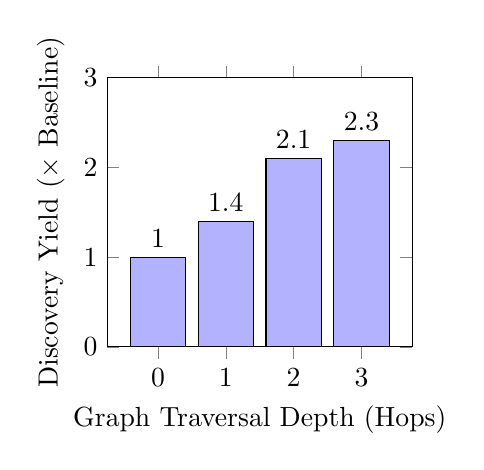
\begin{tikzpicture}
\begin{axis}[
    ybar,
    enlarge x limits=0.25,
    legend style={at={(0.5,-0.15)}, anchor=north, legend columns=-1},
    ylabel={Discovery Yield ($\times$ Baseline)},
    xlabel={Graph Traversal Depth (Hops)},
    symbolic x coords={0, 1, 2, 3},
    xtick=data,
    nodes near coords,
    nodes near coords align={vertical},
    ymin=0, ymax=3,
    width=0.45\textwidth,
    height=5cm,
    bar width=20pt,
]
\addplot[fill=blue!30] coordinates {(0,1.0) (1,1.4) (2,2.1) (3,2.3)};
\end{axis}
\end{tikzpicture}
